\section*{Đề thi thử THPTQG Chuyên Đại học Vinh - Nghệ An 25--26, Lần 1}

\caulc
\Opensolutionfile{ans}[ans/ans-26-2--NgheAn-ChuyenVinh-L1-LC]
\begin{ex}%[Thi thử TN THPT chuyên Đại học Vinh, Nghệ An lần 1, Huỳnh Xuân Tín]%[2D4N1-3]
Họ các nguyên hàm của hàm số $f(x)=2 \sin x+1$ trên $\mathbb{R}$ là
\choice
{$2 \cos x$}
{\True $-2 \cos x+x+C$}
{$2 \cos x+x+C$}
{$-2 \cos x+1+C$}
\loigiai{
Họ các nguyên hàm của hàm số $f(x)=2 \sin x+1$ trên $\mathbb{R}$ là $-2\cos x + x +C$.
}
\end{ex}
\begin{ex}%[Thi thử TN THPT chuyên Đại học Vinh, Nghệ An lần 1, Huỳnh Xuân Tín]%[2H5N2-3]
Trong không gian với hệ trục tọa độ $Oxyz$, đường thẳng $d$ đi qua điểm $M(-1; 4; 6)$, nhận $\overrightarrow{u}=(3; -2; 7)$ làm véc-tơ chỉ phương có phương trình là
\choice
{$\dfrac{x-3}{-1}=\dfrac{y+2}{4}=\dfrac{z-7}{6}$}
{$\dfrac{x-1}{3}=\dfrac{y+4}{-2}=\dfrac{z+6}{7}$}
{$\dfrac{x+3}{-1}=\dfrac{y-2}{4}=\dfrac{z+7}{6}$}
{\True  $\dfrac{x+1}{3}=\dfrac{y-4}{-2}=\dfrac{z-6}{7}$}
\loigiai{
Đường thẳng $d$ đi qua điểm $M(-1; 4; 6)$, nhận $\overrightarrow{u}=(3; -2; 7)$ làm một véc-tơ chỉ phương có phương trình chính tắc là $$\dfrac{x+1}{3}=\dfrac{y-4}{-2}=\dfrac{z-6}{7}.$$
}
\end{ex}
\begin{ex}%[Thi thử TN THPT chuyên Đại học Vinh, Nghệ An lần 1, Huỳnh Xuân Tín]%[1D2N3-2]
Cho cấp số nhân $\left(u_n\right)$ thỏa mãn $u_4=u_1\cdot 8$. Công bội $q$ của $\left(u_n\right)$ bằng
\choice
{$3$}
{\True $2$}
{$-2$}
{$-3$}
\loigiai{
Ta có $u_4=u_1\cdot q^3=u_1\cdot 8\Rightarrow q^3=8\Leftrightarrow q=2$.\\
Vậy công bội của cấp số nhân bằng $2$.}
\end{ex}
\begin{ex}%[Thi thử TN THPT chuyên Đại học Vinh, Nghệ An lần 1, Huỳnh Xuân Tín]%[2D4N3-1]
\immini{Cho hàm số $y=f(x)$ có đạo hàm là $f'(x)$ liên tục trên $[-2; 3]$. Hàm số $y=f'(x)$ có đồ thị như hình vẽ bên.
Biết $\displaystyle\int\limits_{-2}^1 f'(x) \mathrm{\,d}x=3$ và diện tích $S=\dfrac{5}{3}$. Giá trị $f(3)-f(-2)$ bằng
\choice
{$\dfrac{4}{3}$}
{$\dfrac{14}{3}$}
{$-\dfrac{4}{3}$}
{$-\dfrac{14}{3}$}}
{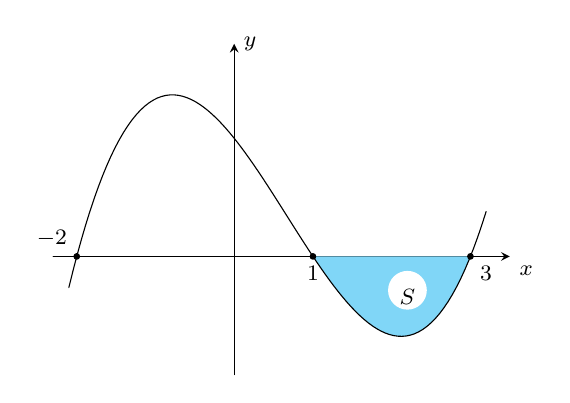
\begin{tikzpicture}[scale=1.0, font=\footnotesize, line join=round, line cap=round, >=stealth]
\draw[->] (-2.3,0)--(3.5,0) node[below right] {$x$};;
\draw[->] (0,-1.5)--(0,2.7) node[right] {$y$};
\fill[cyan!50](1,0)--plot[domain=1:3](\x,{0.25*(\x+2)*(\x-1)*(\x-3)})--(3,0)--cycle;
\draw[samples=100,domain=-2.1:3.2] plot (\x,{0.25*(\x+2)*(\x-1)*(\x-3)});
\draw[fill=black] (1,0) circle(1pt)node[below]{$1$}(3,0) circle(1pt)node[below right]{$3$}(-2,0) circle(1pt)node[above left]{$-2$};
\fill[white] (2.2,-0.43) circle (7pt);
\path (2.2,-0.3) node[below]{$S$};
\end{tikzpicture}}
\loigiai{
Ta có $f(3)-f(-2)=\displaystyle\int\limits_{-2}^3 f'(x) \mathrm{\,d}x=\displaystyle\int\limits_{-2}^1 f'(x) \mathrm{\,d}x+\displaystyle\int\limits_{1}^3 f'(x) \mathrm{\,d}x=3-\dfrac{5}{3}=\dfrac{4}{3}.$\\
}
\end{ex}
\begin{ex}%[Thi thử TN THPT chuyên Đại học Vinh, Nghệ An lần 1, Huỳnh Xuân Tín]%[1H8N7-4]
\immini{Cho lăng trụ đứng $ABC.A'B'C'$ có đáy $ABC$ là tam giác vuông tại $A$ và $BC=2a$, $AA'=2\sqrt{3}a$, $\widehat{ABC}=60^\circ$. Thể tích của khối lăng trụ đã cho bằng
\choice
{$6a^3$}
{$a^3$}
{$2a^3$}
{\True $3a^3$}}
{\begin{tikzpicture}[scale=0.6, font=\footnotesize, line join=round, line cap=round, >=stealth]
\def\a{3.5} \def\b{2} \def\h{3}
\path 
(0:0) coordinate (A)
(130:\b) coordinate (B)
(30:\a) coordinate (C)
(90:\h) coordinate (v)
($(A)+(v)$) coordinate (A')
($(B)+(v)$) coordinate (B')
($(C)+(v)$) coordinate (C')
;
\draw (B)--(A)--(C)
(A')--(B')--(C')--(A')--(A) (C)--(C') (B)--(B');
\draw[dashed](B)--(C);
\foreach \i/\g in {A'/-150,A/-90,B/180,C/0,B'/110,C'/0}{\draw[fill](\i) circle (1.2pt) ($(\i)+(\g:3mm)$) node{$\i$};}
\end{tikzpicture}
}
\loigiai{Do tam giác $ABC$ vuông tại $A$ có $\widehat{ABC}=60^\circ$ và $BC=2a$ nên \\
$AB=BC\cdot\cos\widehat{ABC}=2a\cdot\cos 60^\circ=a\Rightarrow AC=\sqrt{BC^2-AB^2}=a\sqrt{3}$.\\
Vậy $V_{ABC.A'B'C'}=AA'\cdot S_{\triangle ABC}=AA'\cdot\dfrac{1}{2}{AB}\cdot AC=2\sqrt{3}a\cdot\dfrac{1}{2}\cdot a\cdot a\sqrt{3}=3a^3.$}
\end{ex}

\begin{ex}%[Thi thử TN THPT chuyên Đại học Vinh, Nghệ An lần 1, Huỳnh Xuân Tín]%[2D6N1-1]
Cho $\mathrm{P}(A)$, $\mathrm{P}(B)>0$. Công thức xác suất có điều kiện của biến cố $A$ khi biết biến cố $B$ đã xảy ra là
\choice
{$\mathrm{P}\left(A\mid B\right)=\dfrac{\mathrm{P}\left(AB\right)}{\mathrm{P}(A)}$}
{$\mathrm{P}\left(A\mid B\right)=\dfrac{\mathrm{P}(B)}{\mathrm{P}(A)}$}
{\True $\mathrm{P}\left(A\mid B\right)=\dfrac{\mathrm{P}\left(AB\right)}{\mathrm{P}(B)}$}
{$\mathrm{P}\left(A\mid B\right)=\dfrac{\mathrm{P}(A)}{\mathrm{P}(B)}$}
\loigiai{
Ta có $\mathrm{P}\left(A\mid B\right)=\dfrac{\mathrm{P}\left(AB\right)}{\mathrm{P}(B)}$.
}
\end{ex}

\begin{ex}%[Thi thử TN THPT chuyên Đại học Vinh, Nghệ An lần 1, Huỳnh Xuân Tín]%[1D1N5-3]
Tập nghiệm của phương trình $\cot x=\sqrt{3}$ là 
\choice
{$S=\left\{\dfrac{\pi}{3}+k2\pi\mid k\in\mathbb{Z}\right\}$}
{\True $S=\left\{\dfrac{\pi}{6}+k\pi\mid k\in\mathbb{Z}\right\}$}
{$S=\left\{\dfrac{\pi}{6}+k2\pi\mid k\in\mathbb{Z}\right\}$}
{$S=\left\{\dfrac{\pi}{3}+k\pi\mid k\in\mathbb{Z}\right\}$}
\loigiai{
Ta có $\cot x=\sqrt{3}=\cot\dfrac{\pi}{6}\Leftrightarrow x=\dfrac{\pi}{6}+k2\pi$, $k\in\mathbb{Z}$.
}
\end{ex}

\begin{ex}%[Thi thử TN THPT chuyên Đại học Vinh, Nghệ An lần 1, Huỳnh Xuân Tín]%[2H2H1-2]
Cho tứ diện $ABCD$ có $M$, $N$, $O$ lần lượt là trung điểm của $AB$, $CD$, $MN$. Phát biểu nào sau đây là đúng?
\choice
{$\overrightarrow{AB}+\overrightarrow{AC}+\overrightarrow{AD}=\overrightarrow{AO}$}
{$\overrightarrow{AB}+\overrightarrow{AC}+\overrightarrow{AD}=2\overrightarrow{AO}$}
{\True $\overrightarrow{AB}+\overrightarrow{AC}+\overrightarrow{AD}=4\overrightarrow{AO}$}
{$\overrightarrow{AB}+\overrightarrow{AC}+\overrightarrow{AD}=3\overrightarrow{AO}$}
\loigiai{
\immini{
Do $M$, $N$ là trung điểm của $AB$ và $CD$ nên $\overrightarrow{AB}=2\overrightarrow{AM}$,  $\overrightarrow{AC}+\overrightarrow{AD}=2\overrightarrow{AN}$.\\
Suy ra $\overrightarrow{AB}+\overrightarrow{AC}+\overrightarrow{AD}=2\overrightarrow{AM}+2\overrightarrow{AN}=2\left(\overrightarrow{AM}+\overrightarrow{AN}\right)=4\overrightarrow{AO}$.}
{\begin{tikzpicture}[scale=0.8, font=\footnotesize, line join=round, line cap=round,>=stealth]
\def\h{3}
\path
(0,0) coordinate (A)
(1.1,-1.2) coordinate (B)
(3.8,0) coordinate (C)
($(B)!0.5!(A)$) coordinate (M)
(90:\h) coordinate (v)
($(M)+(v)$) coordinate (D)
($(C)!0.5!(D)$) coordinate (N)
($(M)!0.5!(N)$) coordinate (O)
;
\draw (D)--(A)--(B)--(C)--(D)--(B);
\draw[dashed] (A)--(C) (M)--(N);
\foreach \p/\q in {A/180,B/-90,C/-90,M/-90,D/90,N/45,O/0}
\fill[black] (\p) circle (1.0pt) ($(\p)+(\q:2.5mm)$) node{$\p$};
\end{tikzpicture}}
}
\end{ex}
\begin{ex}%[Thi thử TN THPT chuyên Đại học Vinh, Nghệ An lần 1, Huỳnh Xuân Tín]%[1D6N3-2]
Tập xác định của hàm số $y=\log_2(3-x)$ là
\choice
{$\mathscr{D}=(-\infty;3]$}
{\True $\mathscr{D}=(-\infty;3)$}
{$\mathscr{D}=(2;3)$}
{$\mathscr{D}=(3;+\infty)$}
\loigiai{
Điều kiện $3-x>0\Leftrightarrow x<3$.\\
Tập xác định của hàm số là $\mathscr{D}=(-\infty;3)$.
}
\end{ex}
\begin{ex}%[Thi thử TN THPT chuyên Đại học Vinh, Nghệ An lần 1, Huỳnh Xuân Tín]%[1H4H4-3]
Cho hình hộp $ABCD.A_1B_1C_1D_1$ có điểm $M$ thuộc đoạn thẳng $AC$ ($M$  không trùng với $A$ hoặc $C$). Đường thẳng $B_1M$ song song với mặt phẳng nào sau đây?
\choice
{$(CDD_1)$}
{\True $(DA_1C_1)$}
{$(ADD_1)$}
{$(BDD_1)$}
\loigiai{
\immini{
Ta có \begin{itemize}
\item Tứ giác $A_1B_1CD$ là hình bình hành nên $B_1C \parallel A_1D \Rightarrow B_1C \parallel (DA_1C_1)$.
\item Tương tự, tứ giác $ACC_1A_1$ là hình bình hành nên $AC \parallel A_1C_1 \Rightarrow AC \parallel (DA_1C_1)$.
\end{itemize}
Mà $\heva{&B_1C \subset (B_1CA) \\&AC \subset (B_1CA)\\
& B_1C \cap AC=C.} \Rightarrow (B_1CA) \parallel(DA_1C_1)$.\\
Do $B_1 M \subset (B_1CA)$ nên $B_1 M \parallel (DA_1C_1)$.
}
{
\begin{tikzpicture}[,scale=1,font=\footnotesize,line join=round,line cap=round,>=stealth]
\path
(0,0) coordinate (B)
(1,0.8) coordinate (A)
(4,0) coordinate (C)
($(C)-(B)+(A)$) coordinate (D)
($(B)!1/3!(D)$) coordinate (H)
($(H)+(90:4)$) coordinate (A_1)
($(B)-(A)+(A_1)$) coordinate (B_1)
($(C)-(A)+(A_1)$) coordinate (C_1)
($(D)-(A)+(A_1)$) coordinate (D_1)
($(A)!0.4!(C)$)coordinate (M)
;
\draw (B_1)--(B)--(C)--(D)--(D_1)--(A_1)--(B_1)--(C_1)--(D_1) (C)--(C_1)--(A_1) (C_1)--(D) (B_1)--(C);
\draw[dashed] (C)--(A)--(D)--(B) (A_1)--(A)--(B) (A_1)--(D) (B_1)--(A);
\draw[red,dashed](B_1)--(M);
\foreach \p/\q in {A/180,B/-135,C/-45,D/0,A_1/90,B_1/180,C_1/-20,D_1/0,M/30}
\fill[black] (\p)node[shift={(\q:3mm)}]{$\p$} circle (1.0pt);
\end{tikzpicture}
}
}
\end{ex}


\begin{ex}%[Thi thử TN THPT chuyên Đại học Vinh, Nghệ An lần 1, Huỳnh Xuân Tín]%[2H5H1-5]
Trong không gian với hệ trục toạ độ $Oxyz$, cho mặt phẳng $(P)$ đi qua $O$ và véc-tơ pháp tuyến $\vec{n}=(2;-2;1)$. Khoảng cách từ điểm $M(3;-1;1)$ đến $(P)$ bằng
\choice
{$9$}
{$1$}
{$\dfrac{5}{3}$}
{\True $3$}
\loigiai{
Phương trình mặt phẳng $(P)$ đi qua $O$ và véc-tơ pháp tuyến $\vec{n}=(2;-2;1)$ là $2x-2y+z=0$.\\
Khi đó khoảng cách từ điểm $M(3;-1;1)$ đến $(P)$ là $$\mathrm{d}\left(M;(P)\right)=\dfrac{|2\cdot 3-2\cdot (-1)+1|}{\sqrt{2^2+(-2)^2+1^2}}=3.$$
}
\end{ex}


\begin{ex}%[Thi thử TN THPT chuyên Đại học Vinh, Nghệ An lần 1, Huỳnh Xuân Tín]%[1D5N2-3]
Cho mẫu số liệu
\begin{center}
\begin{tabular}{|c|c|c|c|c|c|}
\hline
Nhóm& $[6;7)$ & $[7;8)$ & $[8;9)$ & $[9;10)$ & $[10;11)$ \\
\hline
Tần số& $8$ & $12$ & $10$ & $2$ & $3$ \\
\hline
\end{tabular}
\end{center}
Tứ phân vị thứ ba (\textit{làm tròn đến hàng phần trăm}) của mẫu số liệu bằng
\choice
{\True $8{,}63$}
{$7{,}79$}
{$7{,}76$}
{$8{,}57$}
\loigiai{
Ta có $n=35\Rightarrow \dfrac{3\cdot n}{4}=\dfrac{3\cdot 35}{4}=26{,}25\Rightarrow Q_3\in [8;9)$.\\
Khi đó $Q_3=8+\dfrac{26{,}25-(8+12)}{10}\cdot 1=8{,}625\approx 8{,}63$.
}
\end{ex}

\Closesolutionfile{ans}


\cauds
\Opensolutionfile{ans}[ans/ans-26-2--NgheAn-ChuyenVinh-L1-DS]
\begin{ex}%[Thi thử TN THPT chuyên Đại học Vinh, Nghệ An lần 1, Huỳnh Xuân Tín]%[2H5H2-7]
Trong không gian với hệ trục tọa độ $Oxyz$, cho $A(-1; 4; 4)$, $B(-4; 6; 5)$ và đường thẳng \break $d\colon \dfrac{x-2}{2}=\dfrac{y-3}{3}=\dfrac{z+4}{-5}$.
\choiceTF
{\True Hai đường thẳng $AB$ và $d$ chéo nhau}
{Góc giữa hai đường thẳng $AB$ và $d$ bằng $60^{\circ}$}
{\True Khi điểm $C$ thay đổi trên $d$, giá trị nhỏ nhất của diện tích tam giác $ABC$ bằng $\sqrt{42}$}
{\True Đường thẳng vuông góc chung của hai đường thẳng  $AB$ và $d$ đi qua $M(3; 3; 4)$}
\loigiai{
\begin{itemchoice}
\itemch Một véc-tơ chỉ phương của đường thẳng $AB$ là $\overrightarrow{u}_1=\overrightarrow{AB}=(-3; 2; 1)$.\\    
Một véc-tơ chỉ phương của đường thẳng $d$ là $\overrightarrow{u}_2=(2; 3; -5)$ và điểm $D(2; 3;-4) \in d$.\\
Do $2$ véc-tơ $\overrightarrow{u}_1$, $\overrightarrow{u}_2$ không cùng phương nên $AB$, $d$ chéo nhau hoặc  cắt nhau.\\
Lại có $\overrightarrow{A D}=(3; -1; -8)$, $\left[\overrightarrow{u}_1, \overrightarrow{u}_2\right]=(-13; -13; -13)$.\\
Suy ra  $\left[\overrightarrow{u}_1, \overrightarrow{u}_2\right] \cdot \overrightarrow{AD}=78 \neq 0$ nên $3$ véctơ $\overrightarrow{u}_1$, $\overrightarrow{u}_2$, $\overrightarrow{AD}$ không đồng phẳng.\\ Do đó $AB$ và $d$ chéo nhau.
\itemch Gọi $\varphi$ là góc giữa $AB$ và $d$, ta có $\cos \varphi=\dfrac{\left|\overrightarrow{u}_1 \cdot \overrightarrow{u}_2\right|}{\left|\overrightarrow{u}_1\right| \cdot\left|\overrightarrow{u}_2\right|}=\dfrac{|-6+6-5|}{\sqrt{14} \cdot \sqrt{38}}=\dfrac{5}{\sqrt{14} \cdot \sqrt{38}} \neq \dfrac{1}{2} \Rightarrow \varphi \neq 60^{\circ}$.
\itemch Ta có  $S_{\triangle ABC}=\dfrac{1}{2} AB \cdot \mathrm{d}(C, AB)$ trong đó $\mathrm{d}(C, AB)$ là khoảng cách từ $C$ đến $AB$.\\ 
Lại có $AB=\sqrt{14}$ 
không đổi nên $S_{\triangle ABC} $ nhỏ nhất khi $\mathrm{d}(C; AB)$ nhỏ nhất.\\
Khi đó $\mathrm{d}_{\min}(C; AB)=\mathrm{d}(d; AB)=\dfrac{\left|\left[\overrightarrow{u}_1, \overrightarrow{u}_2\right] \cdot \overrightarrow{AD}\right|}{\left|\left[\overrightarrow{u}_1, \overrightarrow{u}_2\right]\right|}=\dfrac{78}{13 \sqrt{3}}=2 \sqrt{3}$.\\
Vậy $\min S_{\triangle ABC}=\dfrac{1}{2} AB \cdot \mathrm{d}(d, AB)=\dfrac{1}{2} \cdot \sqrt{14} \cdot 2 \sqrt{3}=\sqrt{42}$.\\
\itemch Gọi $\Delta$ là đường thẳng vuông góc chung của hai đường thẳng $AB$ và $d$.\\
Gọi $F$ là giao điểm của đường thẳng $\Delta$ và đường thẳng $d$.\\
Vì $F\in d$ nên $F(2+2t_1; 3+3t_1; -4-5t_1)$.\\
Ta có $\overrightarrow{AB}=(-3; 2; 1)$.\\
Do đó phương trình đường thẳng $AB$ là $\heva{&x=-1-3t_2\\&y=4+2t_2\\&z=4+t_2.}$\\
Gọi $G$ là giao điểm  của đường thẳng $\Delta$ và đường thẳng $AB$.\\
Vì $G\in AB$ nên $G(-1-3t_2; 4+2t_2; 4+t_2)$.\\
Ta có $\overrightarrow{FG}=(-3-3t_2-2t_1; 1+2t_2-3t_1; 8+t_2+5t_1)$.\\
Vì $\Delta $ là đường vuông góc chung của $AB$ và $d$ nên
\begin{eqnarray*}
\heva{&\overrightarrow{FG}\cdot \overrightarrow{AB}=0\\&\overrightarrow{FG}\cdot \overrightarrow{u}_d=0}&\Leftrightarrow& \heva{&-3(-3-3t_2-2t_1)+2(1+2t_2-3t_1)+1(8+t_2+5t_1)=0\\&2(-3-3t_2-2t_1)+3(1+2t_2-3t_1)-5(8+t_2+5t_1)=0}\\
& \Leftrightarrow& \heva{&5t_1+14t_2=-19\\&-38t_1-5t_2=43}\\
&\Leftrightarrow &\heva{&t_1=-1\\&t_2=-1.}
\end{eqnarray*} 
Suy ra $F(0;0;1)$ và $G(2;2;3)$.\\
Khi đó $\overrightarrow{FG}=(2;2;2)$.\\
Vậy đường thẳng $\Delta\colon \heva{&x=2t\\&y=2t\\&z=1+2t.}$\\
Thay tọa độ $M(3;3;4)$ vào phương trình đường thẳng $\Delta$, ta được $\heva{&3=2t\\&3=2t\\&4=1+2t}\Leftrightarrow t=\dfrac{3}{2}$.\\ 
Vậy điểm $M$ thuộc đường thẳng $\Delta$.
\end{itemchoice}
}
\end{ex}
\begin{ex}%[Thi thử TN THPT chuyên Đại học Vinh, Nghệ An lần 1, Huỳnh Xuân Tín]%[2D6V2-3]
Nhân dịp năm mới, cô giáo chuẩn bị $40$ bao lì xì may mắn gồm ba loại: loại I có $12$ bao, mỗi bao chứa $50$ nghìn đồng; loại II có $10$ bao, mỗi bao chứa $20$ nghìn đồng; loại III là các bao còn lại, mỗi bao chứa $10$ nghìn đồng. Ba học sinh An, Bình, Chi theo thứ tự lần lượt lên bốc thăm, mỗi người chỉ bốc đúng một bao lì xì và không hoàn lại. \textit{kết quả tính xác suất được làm tròn đến hàng phần trăm}.
\choiceTF
{\True Xác suất An bốc được bao lì xì $10$ nghìn đồng là $0{,}45$}
{\True Xác suất Bình bốc được bao lì xì $10$ nghìn đồng là $0{,}45$}
{\True Biết Bình bốc được bao lì xì $10$ nghìn đồng, xác suất để An bốc được bao lì xì $10$ nghìn đồng là $0{,}44$}
{\True Xác suất để có ít nhất một bạn bốc được bao lì xì $10$ nghìn đồng là $0{,}84$}
\loigiai{
Số bao lì xì $10$ nghìn đồng là $40-12-10=18$ (bao).\\
Gọi $A$, $B$, $C$ lần lượt là các biến cố: \lq \lq Bạn An, Bình, Chi bốc được bao lì xì $10$ nghìn đồng\rq \rq.
\begin{itemchoice}
\itemch Ta có $\mathrm{P}(A)=\dfrac{18}{40}=0{,}45$.
\itemch Nếu An bốc được bao lì xì $10$ nghìn đồng thì $\mathrm{P}(B \mid A)=\dfrac{17}{39}$.\\
Nếu An không bốc được bao lì xì $10$ nghìn đồng thì $\mathrm{P}\left(B \mid \overline{A}\right)=\dfrac{18}{39}$.\\
Xác suất để An không bốc được bao lì xì $10$ nghìn đồng là $\mathrm{P}\left(\overline{A}\right)=\dfrac{22}{40}=\dfrac{11}{20}$.\\
Vậy xác suất để Bình bốc được bao lì xì $10$ nghìn đồng là    
$$
\mathrm{P}(B)=\mathrm{P}(A) \cdot \mathrm{P}(B \mid A)+\mathrm{P}\left(\overline{A}\right) \cdot \mathrm{P}\left(B \mid \overline{A}\right)=\dfrac{9}{20} \cdot \dfrac{17}{39}+\dfrac{11}{20} \cdot \dfrac{18}{39}=\dfrac{9}{20}=0{,}45.
$$
\itemch Xác suất để cả An và Bình đều bốc được bao lì xì $10$ nghìn đồng là $\mathrm{P}(AB)=\mathrm{P}(A)\cdot \mathrm{P}(B)=0{,}45 \cdot \dfrac{17}{39}=\dfrac{51}{260}$.\\
Suy ra $\mathrm{P}(A \mid B)=\dfrac{P(A B)}{P(B)}=\dfrac{\dfrac{51}{260}}{0{,}45}=\dfrac{17}{39} \approx 0{,}44$.
\itemch Ta có $\mathrm{P}\left(\overline{B} \mid \overline{A}\right)=\dfrac{21}{39}=\dfrac{7}{13}$, $\mathrm{P}\left(\overline{C} \mid \overline{AB}\right)=\dfrac{20}{38}=\dfrac{10}{19}$.\\
Xác suất để cả ba bạn đều không bốc được bao lì xì $10$ nghìn đồng là
$$
\mathrm{P}(\overline{ABC})=\dfrac{11}{20} \cdot \dfrac{7}{13} \cdot \dfrac{10}{19}=\dfrac{77}{494}.
$$
Vậy xác suất để có ít nhất một bạn bốc được bao lì xì $10$ nghìn đồng là

$$
1-\dfrac{77}{494}=\dfrac{417}{494} \approx 0{,}84.
$$
\end{itemchoice}
}
\end{ex}
\begin{ex}%[Thi thử TN THPT chuyên Đại học Vinh, Nghệ An lần 1, Huỳnh Xuân Tín]%[0D2H2-2]
Trong mặt phẳng tọa độ $Oxy$, gọi $(S)$ là miền nghiệm của hệ bất phương trình
$$\heva{& x+y\le 4\\& 2x-y\ge 1\\& x\ge 0\\& y\ge 0.}$$
\choiceTF
{Điểm $A(1;2)$ thuộc $S$}
{\True $(S)$ là một miền tam giác}
{Diện tích $(S)$ bằng $\dfrac{49}{6}$}
{Giá trị lớn nhất của biểu thức $P=x+2y$ trên miền $(S)$ bằng $7$}
\loigiai{
\immini{Ta có hệ bất phương trình $\heva{& x+y\le 4\\& 2x-y\ge 1\\& x\ge 0\\& y\ge 0.}$\\
Biểu diễn miền nghiệm của hệ bất phương trình, ta được như hình bên.\\
Miền nghiệm là miền tam giác $BCD$ với $B(0{,}5;0)$, $C\left(\dfrac{5}{3};\dfrac{7}{3}\right)$, $D(4;0)$.
\begin{itemchoice}
\itemch Thay tọa độ điểm $A(1;2)$ vào hệ bất phương trình thì $2\cdot 1-2=0\le 1$ không thỏa mãn nên điểm $A$ không thuộc $S$.
\itemch Theo ở trên thì $(S)$ là một miền tam giác.
\itemch $S_{BCD}=\dfrac{1}{2}\cdot\mathrm{d}\left(C;BD\right)\cdot BD=\dfrac{1}{2}\cdot\dfrac{7}{3}\cdot\left(4-0{,}5\right)=\dfrac{49}{12}$.
\itemch Ta có $P(0{,}5;0)=0{,}5$, $P\left(\dfrac{5}{3};\dfrac{7}{3}\right)=\dfrac{19}{3}$, $P(4;0)=4$.\\
Vậy $\max P=\dfrac{19}{3}$ đạt được tại $C\left(\dfrac{5}{3};\dfrac{7}{3}\right)$.
\end{itemchoice}
}
{\begin{tikzpicture}[line join=round, line cap=round,>=stealth,thick]
\tikzset{every node/.style={scale=0.8}}
\begin{scope}
\clip (-2,-2) rectangle (4.5,5.5);
\fill[pattern=north east lines] (0.5,0)--(4,0)--(1.7,2.3)--(0.5,0)--cycle;
\draw (-0.5,4.5)--(5,-1) node [pos=0.63, above, sloped] {$x+y-4=0$};
\draw (-0.5,-2)--(3,5) node [pos=0.52, above, sloped] {$2x-y=1$};
\end{scope}
\draw[->] (-1,0)--(4.5,0) node[below]{$x$};
\draw[->] (0,-2)--(0,5) node[left]{$y$};
\draw (0,0) node[below right]{$O$};
\foreach \x in {1,2,3,4}
\draw[thin] (\x,1pt)--(\x,-1pt) node [below] {$\x$};
\foreach \y in {-1,1,2,3,4}
\draw[thin] (1pt,\y)--(-1pt,\y) node [left] {$\y$};
\path(1.71,2.33)node[right]{$C$};
\path(0.5,0)node[above left]{$B$};
\path(4,0)node[above right]{$D$};
\end{tikzpicture}}

}
\end{ex}
\begin{ex}%[Thi thử TN THPT chuyên Đại học Vinh, Nghệ An lần 1, Huỳnh Xuân Tín]%[2D1H4-1]
Cho hàm số $f(x)=\dfrac{3x+1}{x+4}$.
\choiceTF
{\True Hàm số $f(x)$ có đạo hàm là $f'(x)=\dfrac{11}{(x+4)^2}$}
{Với $x_1$, $x_2 \in \mathbb{R}$ thoả mãn $x_1<-4<x_2$ thì $f\left(x_1\right)<f\left(x_2\right)$}
{Toạ độ giao điểm của hai đường tiệm cận của đồ thị hàm số là $(3;-4)$}
{\True Giá trị nhỏ nhất của hàm số $f(x)$ trên đoạn $\left[0;1\right]$ bằng $\dfrac{1}{4}$}
\loigiai{
\begin{itemchoice}
\itemch  Ta có $\mathscr{D}=\mathbb{R}\setminus\{-4\}$.\\Ta có $f(x)=\dfrac{3x+1}{x+4} \Rightarrow f'(x)=\dfrac{(3x+1)'(x+4)-(x+4)'(3x+1)}{(x+4)^2}=\dfrac{11}{(x+4)^2}$.
\itemch $f'(x)=\dfrac{11}{(x+4)^2}>0$, $\forall x \neq -4$.\\
Ta có bảng biến thiên như sau
\begin{center}
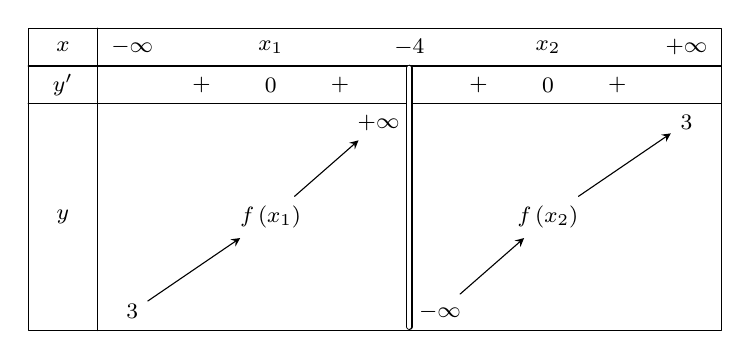
\begin{tikzpicture}[scale=0.8, font=\footnotesize, line join=round, line cap=round,>=stealth,yscale=.6,xscale=1.1]
\def\cot{9} % số nhãn chiều dài
\def\hang{7} % số nhãn chiều cao
\draw[shift={(-.5,.5)}] 
(0,0) rectangle +(\cot+1,-\hang-1)
(0,-1)--+(0:\cot+1) 
(0,-2)--+(0:\cot+1) 
(1,0)--+(-90:\hang+1);
\path 
(0,0) node{$x$} 
(1,0) node{$-\infty$}
(3,0) node{$x_1$}
(5,0) node{$-4$}
(7,0) node{$x_2$}
(9,0) node{$+\infty$} 
(0,-1) node{$y'$}
(2,-1) node{$+$}                                           
(3,-1) node{$0$}
(4,-1) node{$+$}
(6,-1) node{$+$}
(7,-1) node{$0$}
(8,-1) node{$+$}
(0,-4.5) node{$y$}
(1,-7) node (avc) {$3$}
(3,-4.5) node (CD) {$f\left(x_1\right)$} 
(5,-2) node[left] (khongL) {$+\infty$}
(5,-7) node[right] (khongR) {$-\infty$}
(7,-4.5) node (CT) {$f\left(x_2\right)$}
(9,-2) node (dvc) {$3$};
\draw[double, double distance=1.5pt] (5,-0.55)--(5,-7.4); %Không xác định
\draw[->] (avc)--(CD);
\draw[->] (CD)--(khongL);
\draw[->] (khongR)--(CT);
\draw[->] (CT)--(dvc);
\end{tikzpicture}
\end{center}
\noindent
Dựa vào bảng biến thiên ta thấy $f\left(x_1\right)>3$ và $f\left(x_2\right)<3$ nên $f\left(x_1\right)>f\left(x_2\right)$.
\itemch 
Vì $ \lim \limits_{x\to -4^+} f(x)=-\infty$ nên đồ thị hàm số có đường tiệm cận đứng là $x=-4$. \\
Vì $ \lim\limits_{x\to \pm \infty} f(x)=0$ nên
đồ thị hàm số có đường tiệm cận  ngang là $y=3$.\\
Do đó, giao điểm của hai đường tiệm cận của đồ thị hàm số là $(-4;3)$.
\itemch $f'(x)=\dfrac{11}{(x+4)^2}>0$, $\forall x \in [0;1]$.\\
Ta có $f(0)=\dfrac{1}{4}$; $f(1)=\dfrac{4}{5}$.\\
Vậy giá trị nhỏ nhất của hàm số $f(x)$ trên đoạn $[0;1]$ bằng $\dfrac{1}{4}$.
\end{itemchoice}
} 
\end{ex}

\Closesolutionfile{ans}

\caukq
\Opensolutionfile{ans}[ans/ans-26-2--NgheAn-ChuyenVinh-L1-KQ]
\begin{ex}%[Thi thử TN THPT chuyên Đại học Vinh, Nghệ An lần 1, Huỳnh Xuân Tín]%[2D6V1-2]
Có hai chuồng $A$ và $B$. Chuồng $A$ ban đầu có $9$ con dê trắng và $8$ con dê đen. Chuồng $B$ ban đầu có $5$ con dê trắng và $6$ con dê đen. Các con dê được xem như nhau về kích thước và khả năng bị chọn. Người ta bắt ngẫu nhiên đồng thời $3$ con dê từ chuồng $A$ chuyển sang chuồng $B$. Sau đó, từ chuồng $B$ bắt ngẫu nhiên $2$ con dê ra kiểm tra. Biết rằng cả $2$ con dê bắt ra đều là dê trắng. Hỏi xác suất để cả $2$ con dê trắng đó đều là dê chuyển từ chuồng $A$ sang là bao nhiêu phần trăm? (\textit{kết quả làm tròn đến $2$ chữ số ở phần thập phân}).
\loigiai{
Gọi $A_k$ là biến cố \lq \lq Bắt được $k$ con dê trắng từ chuồng $A$ sang chuồng $B$\rq \rq\, với $k \in\{0,1,2,3\}$.\\
$T$ là biến cố \lq \lq Bắt được $2$ con dê trắng từ chuồng $B$ sau khi chuyển từ chuồng $A$ sang\rq \rq
\begin{itemize}
\item \textbf{Trường hợp 1.} $k=3$ ($3$ con dê trắng).\\
Xác suất của biến cố $A_3$ là $\mathrm{P}\left(A_3\right)=\dfrac{\mathrm{C}_9^3}{\mathrm{C}_{17}^3}=\dfrac{21}{170}$.\\
Khi đó chuồng $B$ có $8$ con dê trắng và $6$ con dê đen, xác suất bắt được $2$ con dê trắng là $\dfrac{\mathrm{C}_8^2}{\mathrm{C}_{14}^2}=\dfrac{4}{13}$
\item \textbf{Trường hợp 2.} $k=2$ ($2$ con dê trắng, $1$ con dê đen)\\
Xác suất của biến cố $A_2$ là $\mathrm{P}\left(A_2\right)=\dfrac{\mathrm{C}_9^2 \mathrm{C}_8^1}{\mathrm{C}_{17}^3}=\dfrac{36}{85}$.\\
Khi đó chuồng $B$ có $7$ con dê trắng và $7$ con dê đen, xác suất bắt được $2$ con dê trắng là $\dfrac{\mathrm{C}_7^2}{\mathrm{C}_{14}^2}=\dfrac{3}{13}$.
\item \textbf{Trường hợp 3.} $k=1$ ($1$ con dê trắng, $2$ con dê đen)\\
Xác suất của biến cố $A_1$ là $\mathrm{P}\left(A_1\right)=\dfrac{\mathrm{C}_9^1 \cdot \mathrm{C}_8^2}{\mathrm{C}_{17}^3}=\dfrac{63}{170}$.\\
Khi đó chuồng $B$ có $6$ con dê trắng và $8$ con dê đen, xác xuất bắt được $2$ con dê trắng là $\dfrac{\mathrm{C}_6^2}{\mathrm{C}_{14}^2}=\dfrac{15}{91}$.
\item \textbf{Trường hợp 4.} $k=0$ ($3$ con dê đen)\\
Xác suất của biến cố $A_0$ là $\mathrm{P}\left(A_0\right)=\dfrac{\mathrm{C}_8^3}{\mathrm{C}_{17}^3}=\dfrac{7}{85}$.
\end{itemize}
Khi đó chuồng $B$ có $5$ con dê trắng và $9$ con dê đen, xác xuất bắt được $2$ con dê trắng là $\dfrac{\mathrm{C}_5^2}{\mathrm{C}_{14}^2}=\dfrac{10}{91}$.\\
Như vậy xác suất bắt được $2$ con dê trắng từ chuồng $B$ sau khi chuyển từ chuồng $A$ sang là
$$
\mathrm{P}(T)=\dfrac{21}{170} \cdot \dfrac{4}{13}+\dfrac{36}{85} \cdot \dfrac{3}{13}+\dfrac{63}{170} \cdot \dfrac{15}{91}+\dfrac{7}{85} \cdot \dfrac{10}{91}=\dfrac{7}{34}.
$$
Xác suất bắt được $2$ con dê trắng đều là dê chuyển từ chuồng $A$ sang là
$$\dfrac{\dfrac{21}{170} \cdot \dfrac{\mathrm{C}_3^2}{\mathrm{C}_{14}^2}+\dfrac{36}{85} \cdot \dfrac{\mathrm{C}_2^2}{\mathrm{C}_{14}^2}}{\dfrac{7}{34}} \approx 0{,}0423861 \quad \text{hay}\quad  4{,}24 \%.$$
}
\end{ex}
\begin{ex}%[Thi thử TN THPT chuyên Đại học Vinh, Nghệ An lần 1, Huỳnh Xuân Tín]%[2D1H3-6]
Một doanh nghiệp sản xuất và bán một loại hàng hóa. Gọi $x$ (đơn vị: nghìn sản phẩm, $0<x \leq 30$, $x \in \mathbb{N}$) là số lượng sản phẩm bán ra được. Giá bán mỗi sản phẩm (nghìn đồng/sản phẩm) phụ thuộc số lượng bán ra theo công thức $p(x)=120-2x$. Tổng chi phí sản xuất (triệu đồng) khi sản xuất $x$ nghìn sản phẩm là $C(x)=300+60x+0{,}2x^2+0{,}01x^3$. Tìm $x$ để lợi nhuận doanh nghiệp thu được là lớn nhất?
\shortans[]{$13$}
\loigiai{
Doanh thu khi bán $x$ sản phẩm là $D(x)=x(120-2x)$.\\
Lợi nhuận thu được khi bán $x$ sản phẩm là
\begin{eqnarray*}
L(x)&=&D(x)-C(x)\\
&=&x(120-2x)-\left(300+60x+0{,}2 x^2+0{,}01 x^3\right)\\
&=&-0{,}01x^3-2{,}2x^2+60x-300.\\
L'(x)&=&-0{,}03 x^2-4{,}4 x+60\\
\end{eqnarray*}
$ L'(x)=0 \Leftrightarrow x=\dfrac{20(-11+\sqrt{166})}{3}\approx 12{,}56\in (0;30]$ (do $x>0$).\\
Bảng biến thiên
\begin{center}

\begin{tikzpicture}
\tkzTabInit[nocadre=false, lgt=1.2, espcl=2.5, deltacl=0.6]
{$x$/0.6, $L'(x)$/0.6, $L(x)$/2}
{$0$, $x_0$, $30$}
\tkzTabLine{,+,0,-,}
\tkzTabVar{-/, +/, -/}
\end{tikzpicture}
\end{center}
Ta có $L(12)=85{,}92$, $L(13)=86{,}23$.\\
Vì $x$ nguyên nên $x=13$.\\
Vậy doanh nghiệp bán $13$ sản phẩm thì  lợi nhuận doanh nghiệp thu được là lớn nhất.
}
\end{ex}
\begin{ex}%[Thi thử TN THPT chuyên Đại học Vinh, Nghệ An lần 1, Huỳnh Xuân Tín]%[1H8H5-6]
Một công ty du lịch chuyên tổ chức các Tour trải nghiệm - khám phá, đặt hàng cho một cơ sở sản xuất lều bạt một lô hàng gồm $10$ chiếc lều bạt du lịch giống hệt nhau, hình chóp tứ giác đều mà thể tích trong mỗi chiếc lều là $18$ m$^3$, đơn giá tính theo diện tích bạt sử dụng là $500$ nghìn đồng/m$^2$, (không tính đến đường viền, nếp gấp và lều không may bạt ở đáy). Hỏi số tiền ít nhất mà công ty du lịch phải trả cho cơ sở sản xuất lều bạt là bao nhiêu triệu đồng? (\textit{kết quả làm tròn đến hàng đơn vị}).
\shortans[]{$156$}
\loigiai{\immini{Giả sử chiếc lều có dạng là hình chóp tứ giác đều $S.ABCD$ có đáy $ABCD$ là hình vuông cạnh bằng $2x$.\\
Gọi $O$ là tâm của hình vuông $ABCD$ và $M$ là trung điểm của $AB$.\\
Suy ra $SO\perp(ABCD)$ và $OM\perp AB$, $OM=x$.\\
Do $SO\perp(ABCD)$ và $OM\perp AB\Rightarrow SM\perp AB$.\\
Khi đó $SO=\dfrac{3V_{S.ABCD}}{S_{ABCD}}=\dfrac{3\cdot 18}{(2x)^2}=\dfrac{27}{2x^2}$.}
{\begin{tikzpicture}[scale=0.7, font=\footnotesize, line join=round, line cap=round,>=stealth]
\path
(0,0) coordinate (A)++(-145:2.5) coordinate (B)++(0:4)coordinate (C)
($(A)+(C)-(B)$) coordinate (D)
($(A)!.5!(C)$)coordinate(O)
($(A)!.5!(B)$)coordinate(M)
($(O)+(0,3.5)$) coordinate (S)
;
\draw (S)--(B)--(C)--(D)--cycle (S)--(C);
\draw[dashed] (M)--(O)--(S)--(A)--(D) (C)--(A)--(B)--(D) (S)--(M);
\foreach \p/\q in {S/90,A/-90,B/-90,C/-90,D/0,O/-90,M/-100}
\fill (\p) circle (1.0pt)node[shift={(\q:2.5mm)}]{$\p$};
\end{tikzpicture}}
\noindent Suy ra $SM^2=SO^2+OM^2=\dfrac{27^2}{4x^4}+x^2\Rightarrow S_{SAB}=\dfrac{1}{2}SM\cdot AB=\dfrac{1}{2}\sqrt{\dfrac{27^2}{4x^4}+x^2}\cdot 2x=x\sqrt{\dfrac{27^2}{4x^4}+x^2}$.\\
Do đó diện tích xung quanh của chiếc lều là
$$S_{xq}=4S_{SAB}=4x\sqrt{\dfrac{27^2}{4x^4}+x^2}=4\sqrt{\dfrac{27^2}{4x^2}+x^4}.$$
Xét hàm số $f(t)=\dfrac{27^2}{4t}+t^2$ với $t=x^2>0$.\\
Ta có $f'(t)=2t-\dfrac{27^2}{4t^2}$, suy ra $f'(t)=0\Rightarrow t=\dfrac{9}{2}=4{,}5$.\\
Bảng biến thiên của hàm số $f(t)$ như sau
\begin{center}

\begin{tikzpicture}[line join = round, line cap = round,>=stealth,font=\footnotesize,scale=1]
\tkzTabInit[nocadre=false,lgt=1.2,espcl=2.5,deltacl=0.6]
{$x$ /0.6, $f’(t)$ /0.6, $f(t)$ /2}
{$0$,$4{,}5$,$+\infty$}
\tkzTabLine{ ,-,0,+, }
\tkzTabVar{+/$+\infty$,-/$60{,}75$,+/$+\infty$}
\end{tikzpicture}
\end{center}
Do đó $\min\limits_{\left(0;+\infty\right)}f(t)=60{,}75$ khi $t=\dfrac{9}{2}$, hay $\min S_{xq}=4\sqrt{60{,}75}$ khi $x^2=\dfrac{9}{2}$.\\
Vậy số tiền ít nhất mà công ty du lịch phải trả là
$$ 4\sqrt{60{,}75}\cdot 0{,}5\cdot 10\approx 156 \text{(triệu đồng)}.$$
}
\end{ex}

\begin{ex}%[Thi thử TN THPT chuyên Đại học Vinh, Nghệ An lần 1, Huỳnh Xuân Tín]%[0D8H2-6]
Xét một đa giác đều có $60$ đỉnh. Có bao nhiêu đa giác đều có các đỉnh là một trong các đỉnh của đa giác đều đã cho?
\shortans[]{$78$}
\loigiai{Số đỉnh của mỗi đa giác đều có các đỉnh là một trong các đỉnh của đa giác đều $60$ đỉnh đều phải là ước của $60$.\\
Do $60=2^2\cdot 3\cdot 5$ và số đỉnh của đa giác đều lớn hơn $2$ nên ta có các trường hợp sau
\begin{itemize}
\item \textbf{Trường hợp 1.} Số đỉnh của đa giác đều là số nguyên tố.\\
Khi đó số đa giác đều thỏa mãn là $2^2\cdot 5+2^2\cdot 3=32$.
\item \textbf{Trường hợp 2.} Số đỉnh của đa giác đều là tích hai ước nguyên tố của $60$.\\
Khi đó số đa giác đều thỏa mãn là $3\cdot 5+2\cdot 5+2\cdot 3+2^2=35$.
\item \textbf{Trường hợp 3.} Số đỉnh của đa giác đều là tích của ba ước nguyên tố của $60$.\\
Khi đó số đa giác đều thỏa mãn là $5+3+2=10$.
\item \textbf{Trường hợp 4.} Số đỉnh của đa giác đều bằng $60$. Khi đó số đa giác đều thỏa mãn là $1$.\\
Vậy tổng số đa giác đều thỏa mãn là $32+35+10+1=78$.
\end{itemize}
}
\end{ex}
\begin{ex}%[Thi thử TN THPT chuyên Đại học Vinh, Nghệ An lần 1, Huỳnh Xuân Tín]%[2D4V3-3] 
\immini{Một cơ sở sản xuất thiết bị cứu hộ chế tạo một chiếc phao cứu sinh như hình minh họa. Khi đó, theo mặt cắt qua tâm, người ta thấy bán kính ngoài của phao là $R=35$ cm, bán kính trong của phao là $r=25$ cm. Phao được làm từ một loại vật liệu đồng chất, có khối lượng riêng bằng $D=0{,}05$ g/cm$^3$ (coi phao là khối đặc, không có khoang rỗng bên trong). Tính khối lượng của chiếc phao (đơn vị kg), \textit{biết kết quả làm tròn đến hàng phần trăm, số $\pi$ nhận giá trị bằng $3{,}1416$.}
\shortans{$0{,}74$}}
{\tdplotsetmaincoords{60}{120}
\begin{tikzpicture}[tdplot_main_coords, scale=0.7]
% Định nghĩa dải màu
\definecolor{color1}{RGB}{255, 230, 0}
\definecolor{color2}{RGB}{255, 140, 0}
\definecolor{color3}{RGB}{255, 80, 150}
\definecolor{color4}{RGB}{0, 191, 255}
\definecolor{color5}{RGB}{144, 238, 144}

\def\R{2}    % Bán kính lớn
\def\r{0.7}  % Bán kính ống
\def\stepA{10} % Bước nhảy góc quay lớn (độ rộng múi)
\def\stepB{15} % Bước nhảy góc quay nhỏ (độ mịn bề mặt)

% Vẽ từ xa đến gần (Painter's Algorithm) để xử lý che khuất
\foreach \angA in {0,\stepA,...,350}{
\pgfmathsetmacro{\nextA}{\angA+\stepA}

% Chọn màu cho múi hiện tại
\pgfmathsetmacro{\mindex}{int(mod(\angA/20, 5))}
\ifcase\mindex \colorlet{curr}{color1} 
\or \colorlet{curr}{color2}
\or \colorlet{curr}{color3}
\or \colorlet{curr}{color4}
\else \colorlet{curr}{color5} \fi

% Vẽ từng mảnh nhỏ nối giữa 2 lát cắt để tạo độ kín khít
\foreach \angB in {0,\stepB,...,345}{
\pgfmathsetmacro{\nextB}{\angB+\stepB}

% Tọa độ 4 đỉnh của một mảnh bề mặt
\fill[curr, draw=curr!80!black, line width=0.01pt] 
({(\R + \r*cos(\angB))*cos(\angA)}, {(\R + \r*cos(\angB))*sin(\angA)}, {\r*sin(\angB)}) --
({(\R + \r*cos(\nextB))*cos(\angA)}, {(\R + \r*cos(\nextB))*sin(\angA)}, {\r*sin(\nextB)}) --
({(\R + \r*cos(\nextB))*cos(\nextA)}, {(\R + \r*cos(\nextB))*sin(\nextA)}, {\r*sin(\nextB)}) --
({(\R + \r*cos(\angB))*cos(\nextA)}, {(\R + \r*cos(\angB))*sin(\nextA)}, {\r*sin(\angB)}) -- cycle;
}
}
\end{tikzpicture}
}


\loigiai{
\begin{center}
\begin{tikzpicture}[scale=1.3, font=\footnotesize, line join=round, line cap=round, >=stealth]
% Trục tọa độ
\draw[->] (-1,0) -- (5,0) node[below] {$x$};
\draw[->] (0,-1.5) -- (0,1.5) node[left] {$y$};
\node at (-0.2,-0.2) {$O$};

% Đường tròn tạo hình xuyến
\draw[thick, blue] (3,0) circle (1);
\draw[dashed] (3,0) -- (3,1) node[midway, right] {$a=5$};
\filldraw (3,0) circle (1pt) node[below] {$b=30$};

% Chú thích R và r
\draw[|<->|] (0,-1.2) -- (2,-1.2) node[midway, fill=white] {$r=25$};
\draw[|<->|] (0,-1.8) -- (4,-1.8) node[midway, fill=white] {$R=35$};

% Miền quay
\node[blue] at (3,1.3) {$(C)$};
\end{tikzpicture}
\end{center}
Ta có, mặt cắt của phao là một hình tròn có bán kính $a = \dfrac{R-r}{2} = \dfrac{35-25}{2} = 5$ (cm).\\
Tâm của hình tròn này cách tâm phao một khoảng $b = \dfrac{R+r}{2} = \dfrac{35+25}{2} = 30$ (cm).\\
Chọn hệ trục tọa độ $Oxy$ sao cho trục $Oy$ là trục đối xứng của phao (hình vẽ trên). \\
Khi đó, chiếc phao được tạo thành khi quay đường tròn $(C)$ tâm $I (30; 0)$, bán kính $a=5$, quanh trục $Oy$.\\
Phương trình đường tròn $(C)$ là $(x-30)^2 + y^2 = 5^2$.\\
Đường tròn $(C)$ gồm hai cung $x = 30 - \sqrt{25-y^2}$ (cung gần trục $Oy$) và $x = 30 + \sqrt{25-y^2}$ (cung xa trục $Oy$), với $y \in [-5; 5]$.\\
Khi quay hình tròn $(C)$ quanh trục $Oy$ ta được khối tròn xoay (hình chiếc phao theo yêu cầu).\\ 
Thể tích vật thể tròn xoay quanh trục $Oy$ được tính theo công thức
\begin{eqnarray*}
V & = & \pi \displaystyle \int \limits_{-5}^{5} \left[ \left( 30 + \sqrt{25-y^2} \right)^2 - \left( 30 - \sqrt{25-y^2} \right)^2 \right] \mathrm{\,d}y \\
&=& \pi \displaystyle \int \limits_{-5}^{5} \left[ (900 + 60\sqrt{25-y^2} + 25-y^2) - (900 - 60\sqrt{25-y^2} + 25-y^2) \right] \mathrm{\,d}y\\
&=& \pi \displaystyle \int \limits_{-5}^{5} 120\sqrt{25-y^2} \mathrm{\,d}y = 120\pi \displaystyle \int \limits_{-5}^{5} \sqrt{25-y^2} \mathrm{\,d}y.
\end{eqnarray*}
Biểu thức $\displaystyle \int \limits_{-5}^{5} \sqrt{25-y^2} \mathrm{\,d}y$ chính là diện tích nửa hình tròn bán kính $5$, bằng $\dfrac{1}{2} \pi \cdot 5^2 = \dfrac{25\pi}{2}$.\\
Do đó $V = 120\pi \cdot \dfrac{25\pi}{2} = 1\,500\pi^2$ (cm$^3$).\\
Sử dụng $\pi = 3{,}1416$, khi đó 
$V = 1500 \cdot (3{,}1416)^2 \approx 14\,804{,}43$ (cm$^3$).\\
Khối lượng $m = D \cdot V = 0{,}05 \cdot 14\,804{,}43 = 740{,}2215$ (g). Suy ra $m \approx 0{,}74$ kg.
}
\end{ex}

\begin{ex}%[Thi thử TN THPT chuyên Đại học Vinh, Nghệ An lần 1, Huỳnh Xuân Tín]%[1H8V6-2]
Cho hình chóp $S.ABC$ có $SA \perp (ABC)$ và $SA = \sqrt{5}$, $AB = \sqrt{2}$, $BC = 2$, $\widehat{ABC} = 135^\circ$. Số đo của góc nhị diện $[A,SC,B]$ bằng $m^\circ$. Giá trị của $m$ bằng bao nhiêu? (\textit{Kết quả làm tròn đến hàng đơn vị}).
\shortans{$30$}
\loigiai{
\immini{
Gọi $H$ là hình chiếu của $A$ lên $BC$; $K, I$ lần lượt là hình chiếu của $A$ lên $SH$ và $SC$.\\
Ta có $\heva{&HC\perp AH\\&HC\perp SA}\Rightarrow HC\perp (SAH)$.\\
Từ đó $\heva{&AK\perp SH\\&AK\perp HC,\,\text{ do } HC\perp (SAH)}\Rightarrow AK\perp (SHC)$.\\
Vậy $\heva{&SC\perp AI\\&SC\perp AK}\Rightarrow SC\perp (AKI)$, suy ra $[A,SC,B]=\widehat{AIK}$.\\ 
Khi đó ta có $AH = \dfrac{AB}{\sqrt{2}} = 1$ vì tam giác $ABH$ vuông cân tại $H$.\\
Lại có $AK = \dfrac{SA \cdot AH}{\sqrt{SA^2 + AH^2}} = \dfrac{\sqrt{30}}{6}$;\\
$AC = \sqrt{BA^2 + BC^2 - 2BA \cdot BC \cdot \cos\widehat{ABC}} = \sqrt{10}$;\\
$AI = \dfrac{SA \cdot AC}{\sqrt{SA^2 + AC^2}} = \dfrac{\sqrt{30}}{3}$.\\
Suy ra $\sin \widehat{AIK} = \dfrac{AK}{AI} = \dfrac{1}{2} \Leftrightarrow \widehat{AIK} = 30^\circ$.\\
Vậy $[A, SC, B] = \widehat{AIK} = 30^\circ$.
}{
\begin{tikzpicture}[scale=1, font=\footnotesize, line join=round, line cap=round,>=stealth]
\path
(0,0) coordinate (A)
(1.2,-1.5) coordinate (H)
(4,0) coordinate (C)
($(A)+(0,3.3)$) coordinate (S)
($(H)!0.35!(C)$) coordinate (B)
($(S)!0.35!(C)$) coordinate (I)
($(S)!0.6!(H)$) coordinate (K)
;
\draw (S)--(A) (B)--(C)--(S) (S)--(B) (S)--(H) (I)--(K) (A)--(H)--(B) (A)--(K);
\draw[dashed] (A)--(C) (I)--(A)--(H)  (A)--(B);
\foreach \p/\q in {S/90,A/180,B/-90,C/0,H/-90,K/30,I/90}
\fill[black] (\p) circle (1.0pt) ($(\p)+(\q:2.5mm)$) node{$\p$};
\draw pic[draw=black,angle radius=0.2cm] {right angle = S--A--C};
\draw pic[draw=black,angle radius=0.2cm] {right angle = S--A--H}; 
\draw pic[draw=black,angle radius=0.2cm] {right angle = A--H--B};
\draw pic[draw=black,angle radius=0.2cm] {right angle = A--I--S};
\draw pic[draw=black,angle radius=0.2cm] {right angle = A--K--H};
\end{tikzpicture}
}
}
\end{ex}


\Closesolutionfile{ans}

\indapan{6}{ans/ans-26-2--NgheAn-ChuyenVinh-L1-LC}
\indapan{4}{ans/ans-26-2--NgheAn-ChuyenVinh-L1-DS}
\indapan{6}{ans/ans-26-2--NgheAn-ChuyenVinh-L1-KQ}
